% THIS IS SIGPROC-SP.TEX - VERSION 3.1
% WORKS WITH V3.2SP OF ACM_PROC_ARTICLE-SP.CLS
% APRIL 2009
%
% It is an example file showing how to use the 'acm_proc_article-sp.cls' V3.2SP
% LaTeX2e document class file for Conference Proceedings submissions.
% ----------------------------------------------------------------------------------------------------------------
% This .tex file (and associated .cls V3.2SP) *DOES NOT* produce:
%       1) The Permission Statement
%       2) The Conference (location) Info information
%       3) The Copyright Line with ACM data
%       4) Page numbering
% ---------------------------------------------------------------------------------------------------------------
% It is an example which *does* use the .bib file (from which the .bbl file
% is produced).
% REMEMBER HOWEVER: After having produced the .bbl file,
% and prior to final submission,
% you need to 'insert'  your .bbl file into your source .tex file so as to provide
% ONE 'self-contained' source file.
%
% Questions regarding SIGS should be sent to
% Adrienne Griscti ---> griscti@acm.org
%
% Questions/suggestions regarding the guidelines, .tex and .cls files, etc. to
% Gerald Murray ---> murray@hq.acm.org
%
% For tracking purposes - this is V3.1SP - APRIL 2009

\documentclass{acm_proc_article-sp}

\usepackage{caption}
\usepackage{soul}
\usepackage{color}
\usepackage{url}
\usepackage{hyperref}
\usepackage{subfig}
\usepackage{graphicx}
\usepackage{algpseudocode}

\begin{document}
\title{Phylogenetic Trees and Felsenstein's Algorithm}
\subtitle{Assignment 6}
%
% You need the command \numberofauthors to handle the 'placement
% and alignment' of the authors beneath the title.
%
% For aesthetic reasons, we recommend 'three authors at a time'
% i.e. three 'name/affiliation blocks' be placed beneath the title.
%
% NOTE: You are NOT restricted in how many 'rows' of
% "name/affiliations" may appear. We just ask that you restrict
% the number of 'columns' to three.
%
% Because of the available 'opening page real-estate'
% we ask you to refrain from putting more than six authors
% (two rows with three columns) beneath the article title.
% More than six makes the first-page appear very cluttered indeed.
%
% Use the \alignauthor commands to handle the names
% and affiliations for an 'aesthetic maximum' of six authors.
% Add names, affiliations, addresses for
% the seventh etc. author(s) as the argument for the
% \additionalauthors command.
% These 'additional authors' will be output/set for you
% without further effort on your part as the last section in
% the body of your article BEFORE References or any Appendices.

%\numberofauthors{3} %  in this sample file, there are a *total*
% of EIGHT authors. SIX appear on the 'first-page' (for formatting
% reasons) and the remaining two appear in the \additionalauthors section.
%
\numberofauthors{1}
\author{
	\alignauthor Caitlin Ross\\
	\affaddr{Computer Science Department, Rensselaer Polytechnic Institute} \\
	\email{rossc3@rpi.edu}
}
% There's nothing stopping you putting the seventh, eighth, etc.
% author on the opening page (as the 'third row') but we ask,
% for aesthetic reasons that you place these 'additional authors'
% in the \additional authors block, viz.

\date{30 July 1999}
% Just remember to make sure that the TOTAL number of authors
% is the number that will appear on the first page PLUS the
% number that will appear in the \additionalauthors section.

\maketitle

\begin{abstract}
This work implements Felsenstein's algorithm for likelihood using the Jukes-Cantor model as the substitution matrix.  The program is run on three trees with the same species but different branch patterns and lengths.  The algorithm determines the probability of the data given the tree for each tree.  Final results are shown for each tree as well as intermediate probabilities at each node and leaf.  
\end{abstract}


\section{Problem Statement}
The problem here is to implement the Felsenstein algorithm for likelihood and run it on three different phylogentic trees.  The Felsentein algorithm determines the probability of the data given the tree.  


\section{Methods}
Three phylogenetic trees are given for this assignment.  The nodes of the trees show the name of the species with a nucleotide.  All three trees contain the same set of species and nucleotide pairs, but the trees branch differently.  

The Felsenstein algorithm was implemented in order to determine the probability of the data given each tree.  The algorithm is as follows:  \\
\textbf{Initialization:} $k = 2n - 1$ \\
\textbf{Recursion:} Compute $P(L_k | a)$ for all $a$ as follows: 
\begin{algorithmic}
\If{k is leaf node}
\State Set $P(L_k | a) = 1$ if $a = x_u^k$, $P(L_k | a) = 0$ if $ a \neq x_u^k$
\Else
\State compute $P(L_i | a)$, $P(L_j | a)$ for all $a$ at the daughter nodes $i$, $j$
\State $P(L_k | a) = \sum_{b,c} P(b|a, t_i)P(L_i|b)P(c|a,t_j)P(L_j|c)$
\EndIf
\end{algorithmic}
\textbf{Termination:} \\
Likelihood at site u: \\ 
$P(x_u | T,t) = \sum\limits_{a\in \{A,C,G,T\}} P(L_{2n-1} | a)q_a$

In this algorithm $P(b|a, t_i)$ is from the Jukes-Cantor substitution matrix (defined below), where $a,b \in \{A,C,G,T\}$.  $P(L_k | a)$ is the probability that all leaves below node $k$ given $a \in \{A,C,G,T\}$ at $k$. Also, $q_a = .25, \forall a \in \{A,C,G,T\}$.

The Jukes-Cantor substitution matrix is defined as:
 \[ S(t) = \left( \begin{array}{cccc}
r_t & s_t & s_t & s_t \\
s_t & r_t & s_t & s_t \\
s_t & s_t & r_t & s_t \\
s_t & s_t & s_t & r_t \end{array} \right)\]
where 
\begin{equation} r_t = \frac{1}{4}(1+3e^{-4\alpha t})\end{equation}
and
\begin{equation} s_t = \frac{1}{4}(1-e^{-4\alpha t})\end{equation}

The program written for this work reads in the trees, which are given in Newick format.  It then runs the Felsenstein algorithm on each tree.  For each node of the tree, the program reports $P(L_k |a)$ for each nucleotide.  At the end of the recursion, it reports the final P(data|tree), described in the termination step of Felsenstein's algorithm above.  

%\begin{figure}[!b]
%	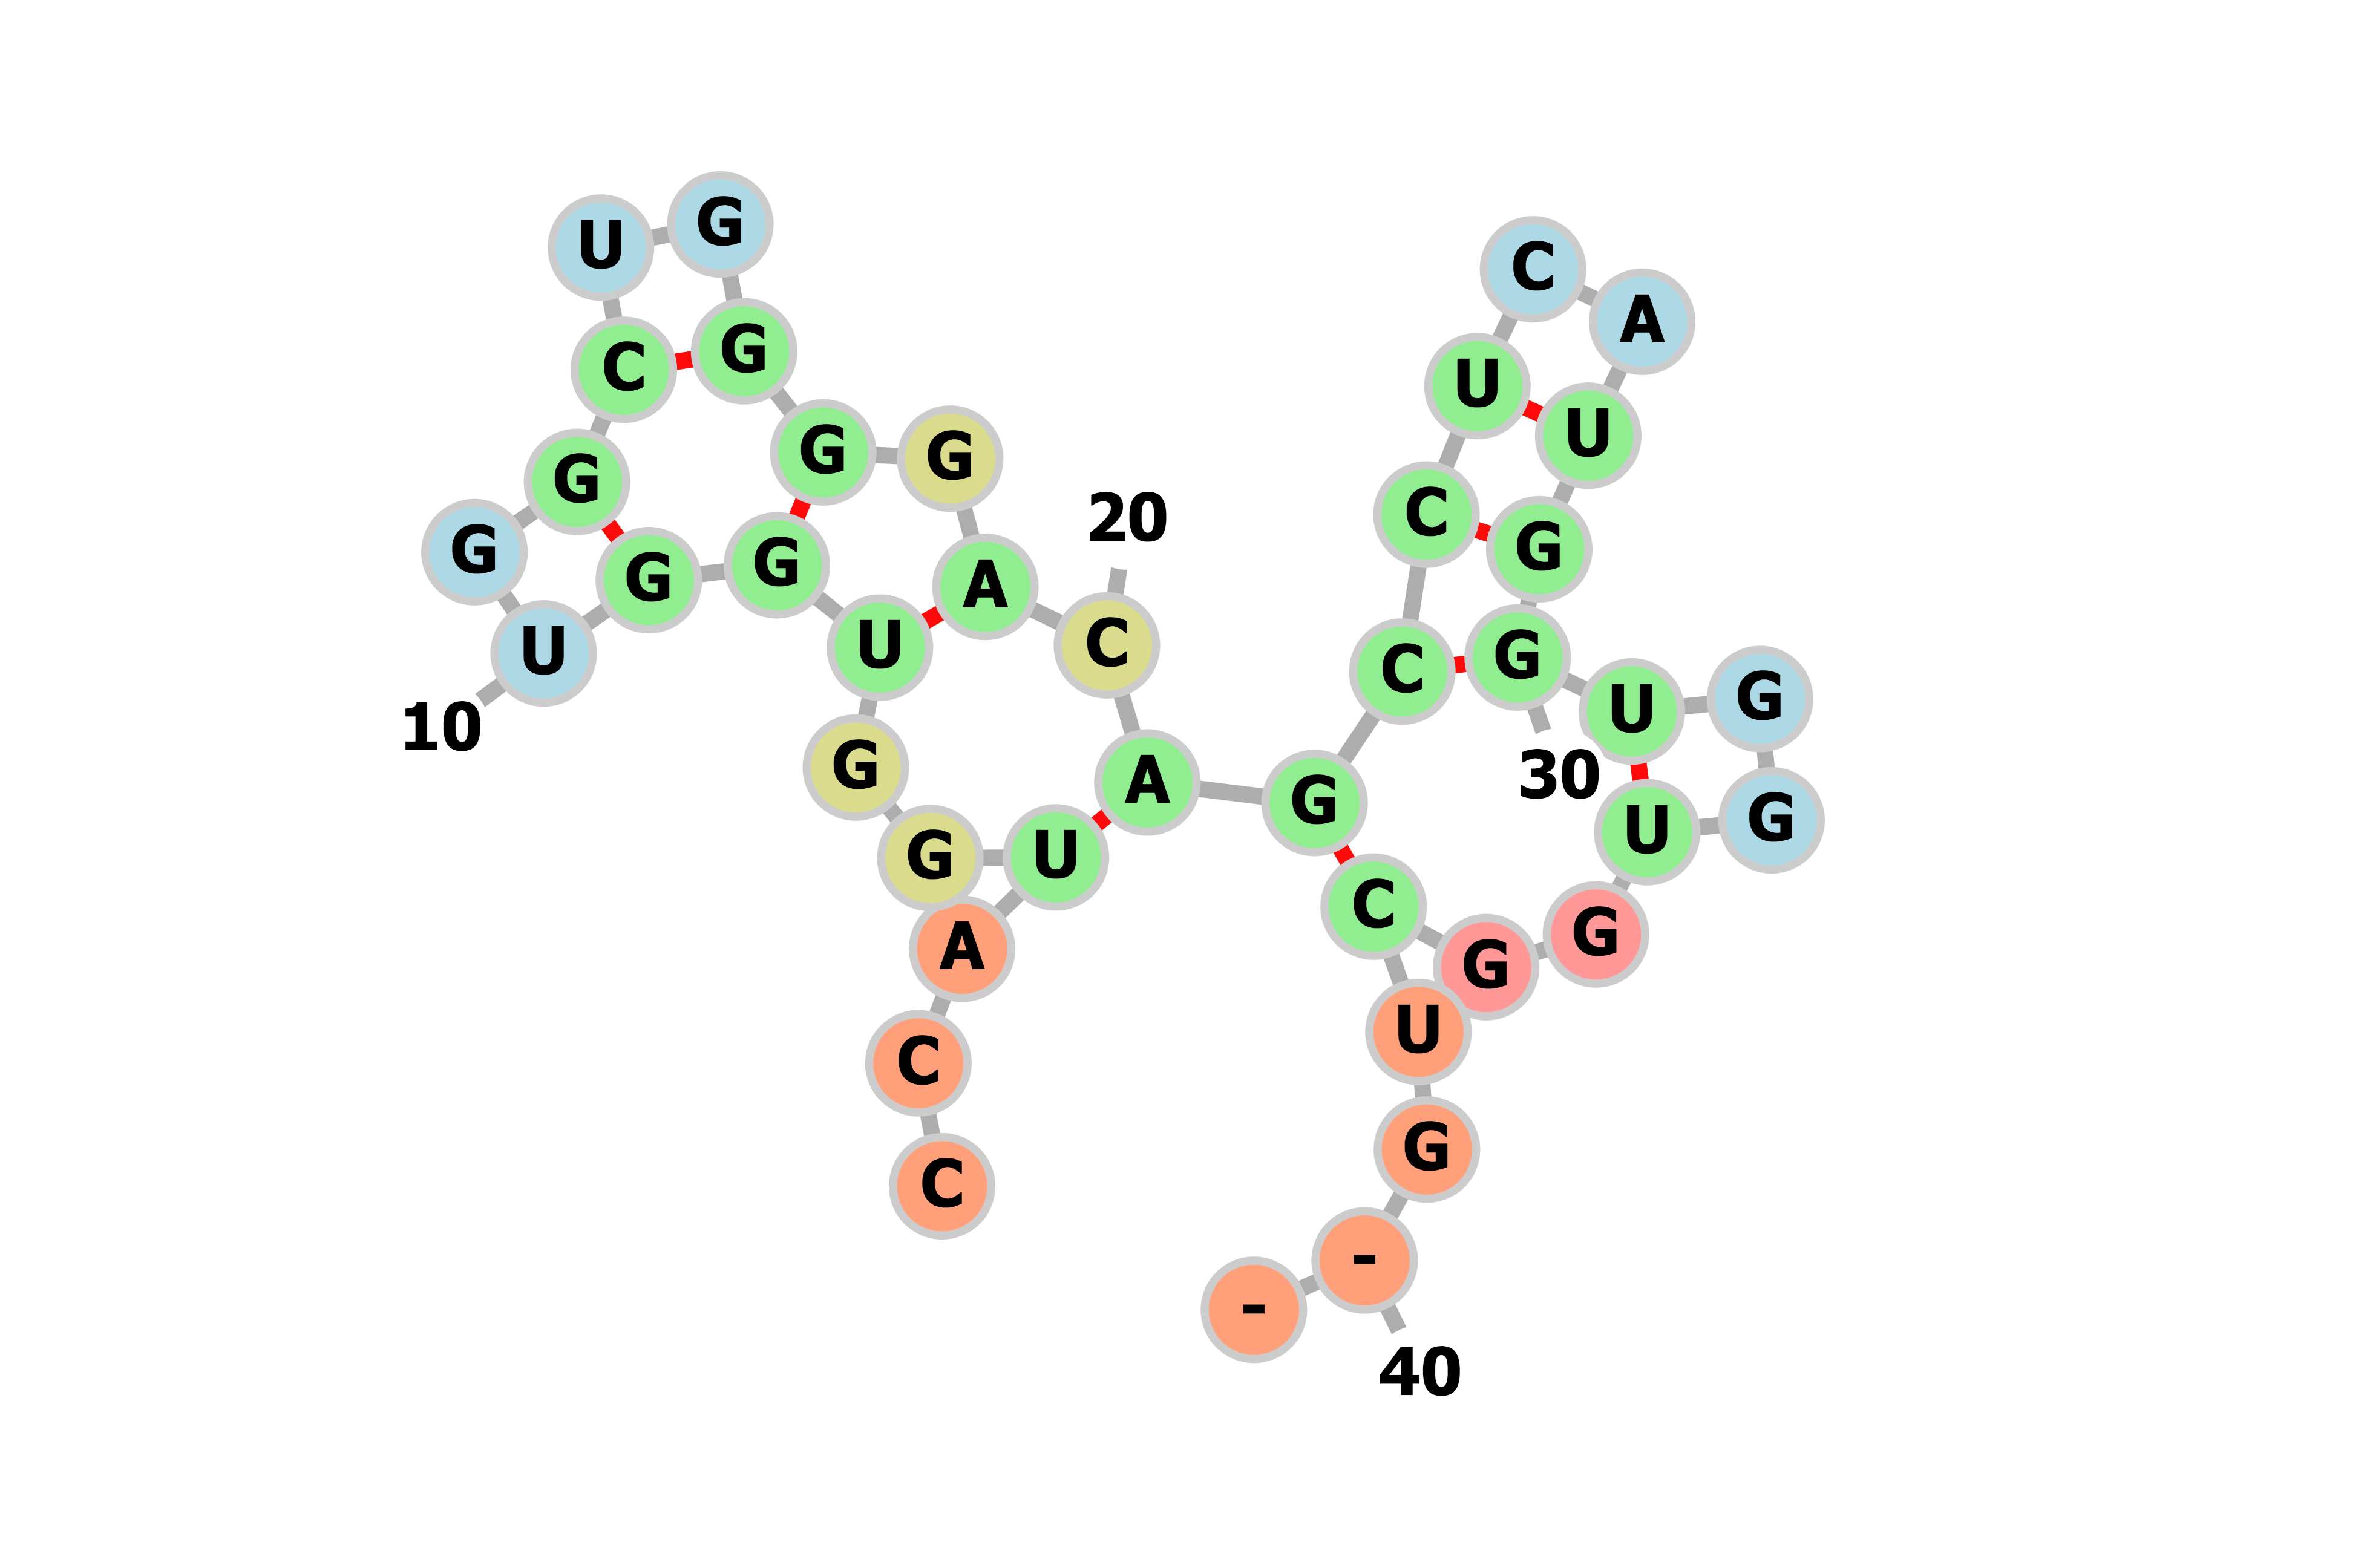
\includegraphics[trim={0 0 2cm 0}, clip,width=3.5in]{rna.png}
%	\caption{Plotted RNA secondary structure for the consensus sequence.}
%	\label{fig:hist}
%\end{figure}

\section{Results}
The results for tree1.txt: \\
probability at leaf A \{'G': 0, 'C': 0, 'T': 0, 'A': 1\}\\
probability at leaf C \{'G': 0, 'C': 1, 'T': 0, 'A': 0\}\\
probability at leaf C \{'G': 0, 'C': 1, 'T': 0, 'A': 0\}\\
probability at leaf C \{'G': 0, 'C': 1, 'T': 0, 'A': 0\}\\
probability at leaf G \{'G': 1, 'C': 0, 'T': 0, 'A': 0\}\\
probability at leaf G \{'G': 1, 'C': 0, 'T': 0, 'A': 0\}\\
probability at node \{'G': 0.999, 'C': 2.297e-08, 'T': 2.297e-08, 'A': 2.297e-08\}\\
probability at node \{'G': 0.000171, 'C': 8.375e-05, 'T': 1.436e-08, 'A': 1.436e-08\}\\
probability at node \{'G': 5.754e-08, 'C': 8.366e-05, 'T': 1.201e-11, 'A': 1.201e-11\}\\
probability at node \{'G': 2.259e-11, 'C': 8.355e-05, 'T': 1.852e-12, 'A': 1.852e-12\}\\
probability at node \{'G': 8.731e-12, 'C': 5.787e-08, 'T': 8.717e-12, 'A': 1.255e-08\}\\
P(data|tree) = 1.761e-08

Results for tree2.txt:\\
probability at leaf A \{'G': 0, 'C': 0, 'T': 0, 'A': 1\} \\
probability at leaf C \{'G': 0, 'C': 1, 'T': 0, 'A': 0\}\\
probability at leaf C \{'G': 0, 'C': 1, 'T': 0, 'A': 0\}\\
probability at leaf C \{'G': 0, 'C': 1, 'T': 0, 'A': 0\}\\
probability at leaf G \{'G': 1, 'C': 0, 'T': 0, 'A': 0\}\\
probability at leaf G \{'G': 1, 'C': 0, 'T': 0, 'A': 0\}\\
probability at node \{'G': 0.999, 'C': 2.297e-08, 'T': 2.297e-08, 'A': 2.297e-08\}\\
probability at node \{'G': 0.000534, 'C': 0.000283, 'T': 1.519e-07, 'A': 1.519e-07\}\\
probability at node \{'G': 3.052e-07, 'C': 0.000282, 'T': 1.258e-10, 'A': 1.258e-10\}\\
probability at node \{'G': 1.163e-10, 'C': 0.000282, 'T': 6.288e-12, 'A': 6.288e-12\}\\
probability at node \{'G': 2.951e-11, 'C': 1.954e-07, 'T': 2.943e-11, 'A': 4.239e-08\}\\
P(data|tree) = 5.947e-08

Results for tree3.txt: \\
probability at leaf A \{'G': 0, 'C': 0, 'T': 0, 'A': 1\}\\
probability at leaf C \{'G': 0, 'C': 1, 'T': 0, 'A': 0\}\\
probability at leaf C \{'G': 0, 'C': 1, 'T': 0, 'A': 0\}\\
probability at node \{'G': 2.058e-07, 'C': 0.997, 'T': 2.058e-07, 'A': 2.058e-07\}\\
probability at leaf C \{'G': 0, 'C': 1, 'T': 0, 'A': 0\}\\
probability at leaf G \{'G': 1, 'C': 0, 'T': 0, 'A': 0\}\\
probability at leaf G \{'G': 1, 'C': 0, 'T': 0, 'A': 0\}\\
probability at node \{'G': 0.999, 'C': 2.297e-08, 'T': 2.297e-08, 'A': 2.297e-08\}\\
probability at node \{'G': 0.000534, 'C': 0.000283, 'T': 1.519e-07, 'A': 1.519e-07\}\\
probability at node \{'G': 4.493e-07, 'C': 0.000281, 'T': 1.8520202918226461e-10, 'A': 1.852e-10\}\\
probability at node \{'G': 3.232e-10, 'C': 1.950e-07, 'T': 1.209e-11, 'A': 1.741e-08\}\\
P(data|tree) = 5.319e-08

Tree 2 has the highest probability out of the three trees given.
%
% The following two commands are all you need in the
% initial runs of your .tex file to
% produce the bibliography for the citations in your paper.
\bibliographystyle{abbrv}
%\bibliography{sigproc}  % sigproc.bib is the name of the Bibliography in this case

% You must have a proper ".bib" file
%  and remember to run:
% latex bibtex latex latex
% to resolve all references
%
% ACM needs 'a single self-contained file'!
%
%APPENDICES are optional
%\balancecolumns

\balancecolumns
% That's all folks!
\end{document}
